% Apêndice com figuras movidas da seção de resultados
% Usamos numeração fixa A.1, A.2, ... para garantir consistência com a classe
\renewcommand{\thefigure}{A.\arabic{figure}}
\setcounter{figure}{0}

\clearpage
\onecolumn
\section*{Apêndice — Figuras Complementares}

% Primeira figura aparece imediatamente após o título (não-flutuante)
\begin{center}
    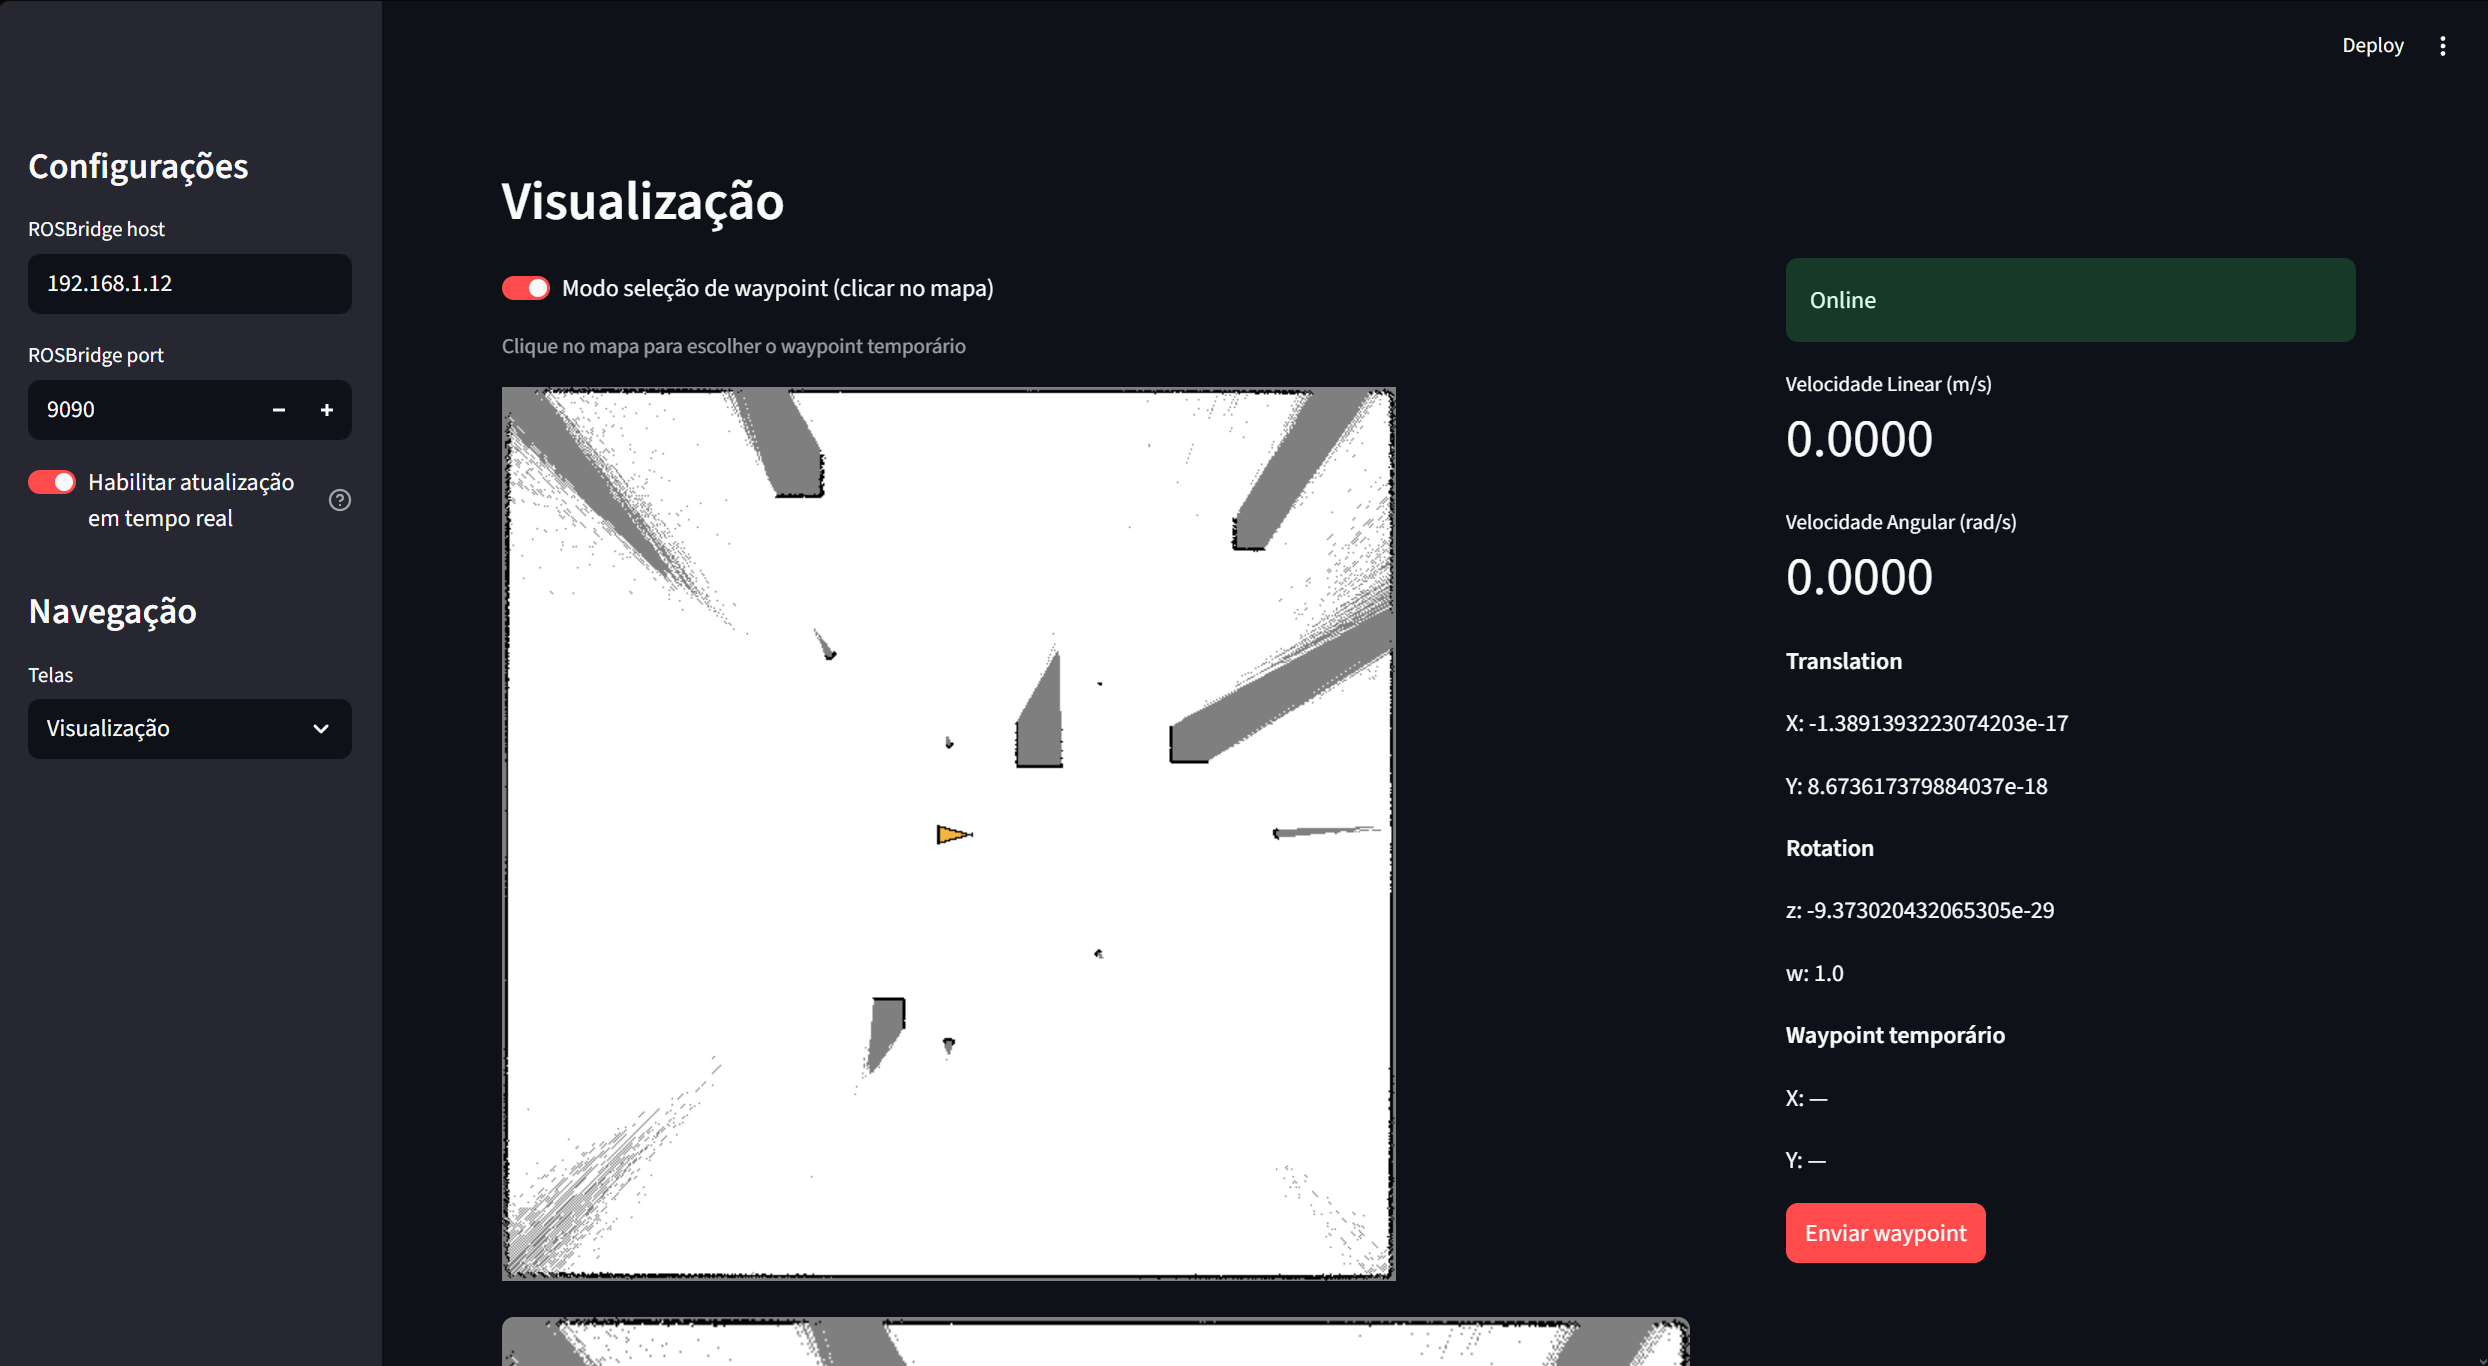
\includegraphics[width=\textwidth]{images/Visualizacao.png}
    \vskip0.5\baselineskip
    \captionof{figure}{Módulo de visualização da interface.}\label{fig:visualizacao}
\end{center}

% Para as figuras seguintes colocamos cada uma em página própria

\begin{center}
    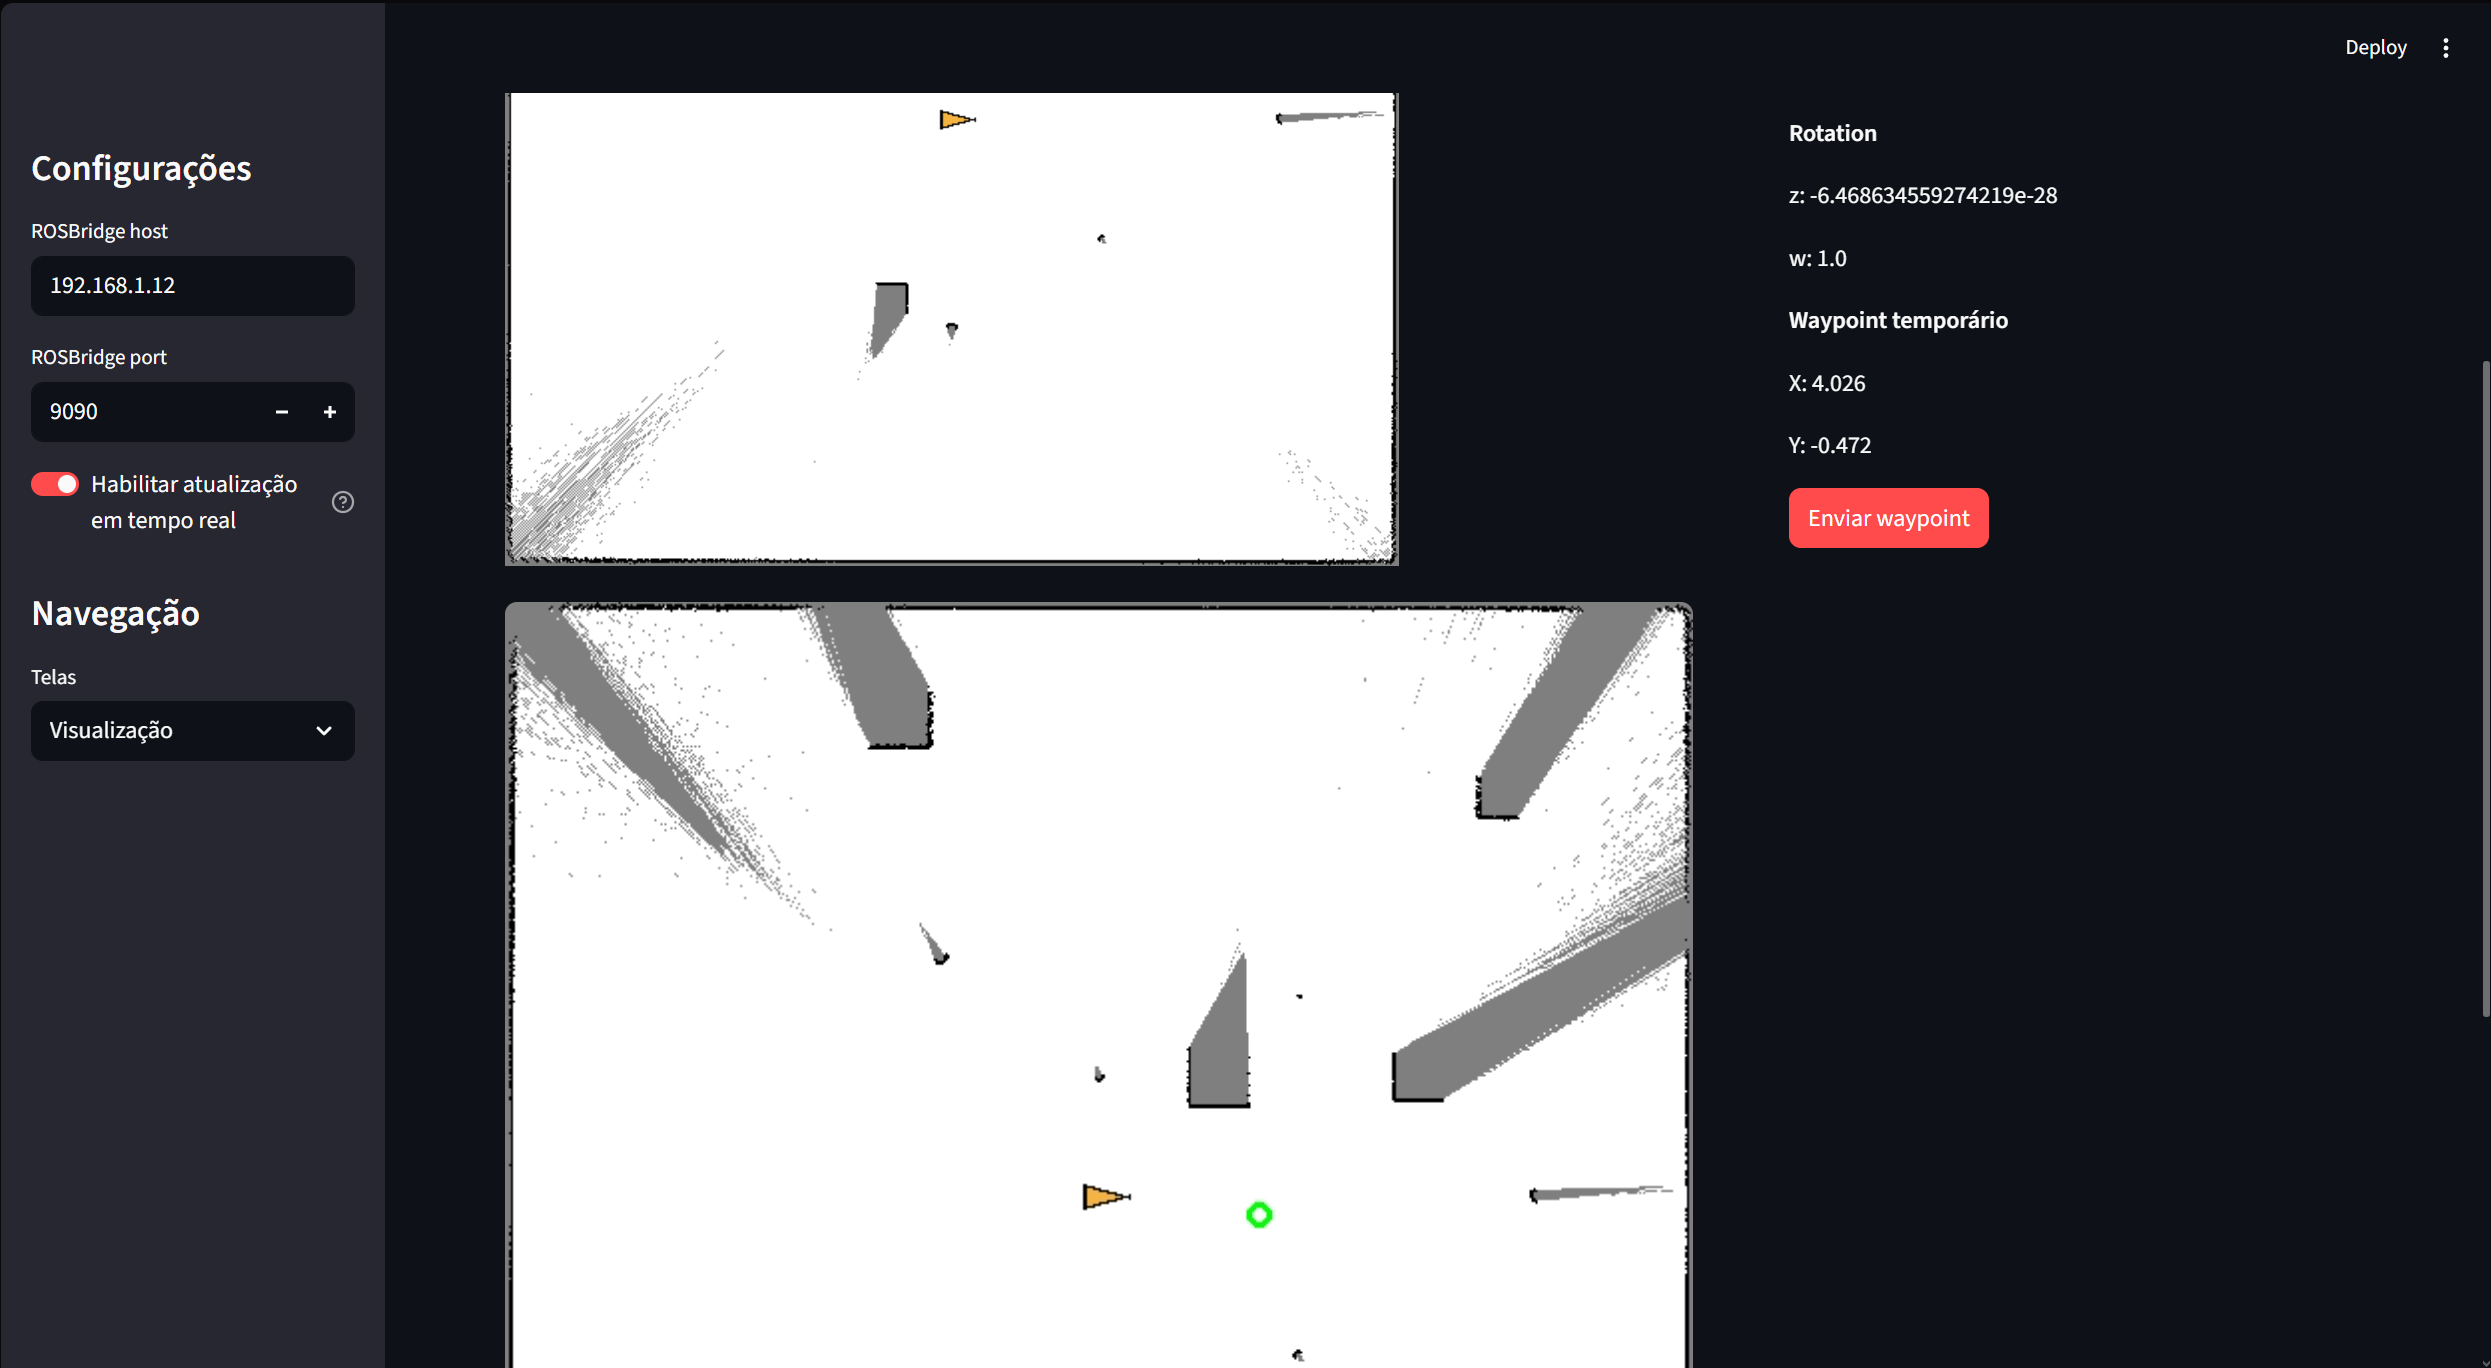
\includegraphics[width=\textwidth]{images/MostraWaypoint.png}
    \vskip0.5\baselineskip
    \captionof{figure}{Funcionalidade de definição de waypoint na interface.}\label{fig:mostra_waypoint}
\end{center}

\begin{center}
    \includegraphics[width=\textwidth]{images/RVizWaypoint.png}
    \vskip0.5\baselineskip
    \captionof{figure}{Envio de waypoint para o ROS e navegação automática do robô.}\label{fig:rvizwaypoint}
\end{center}

\begin{center}
    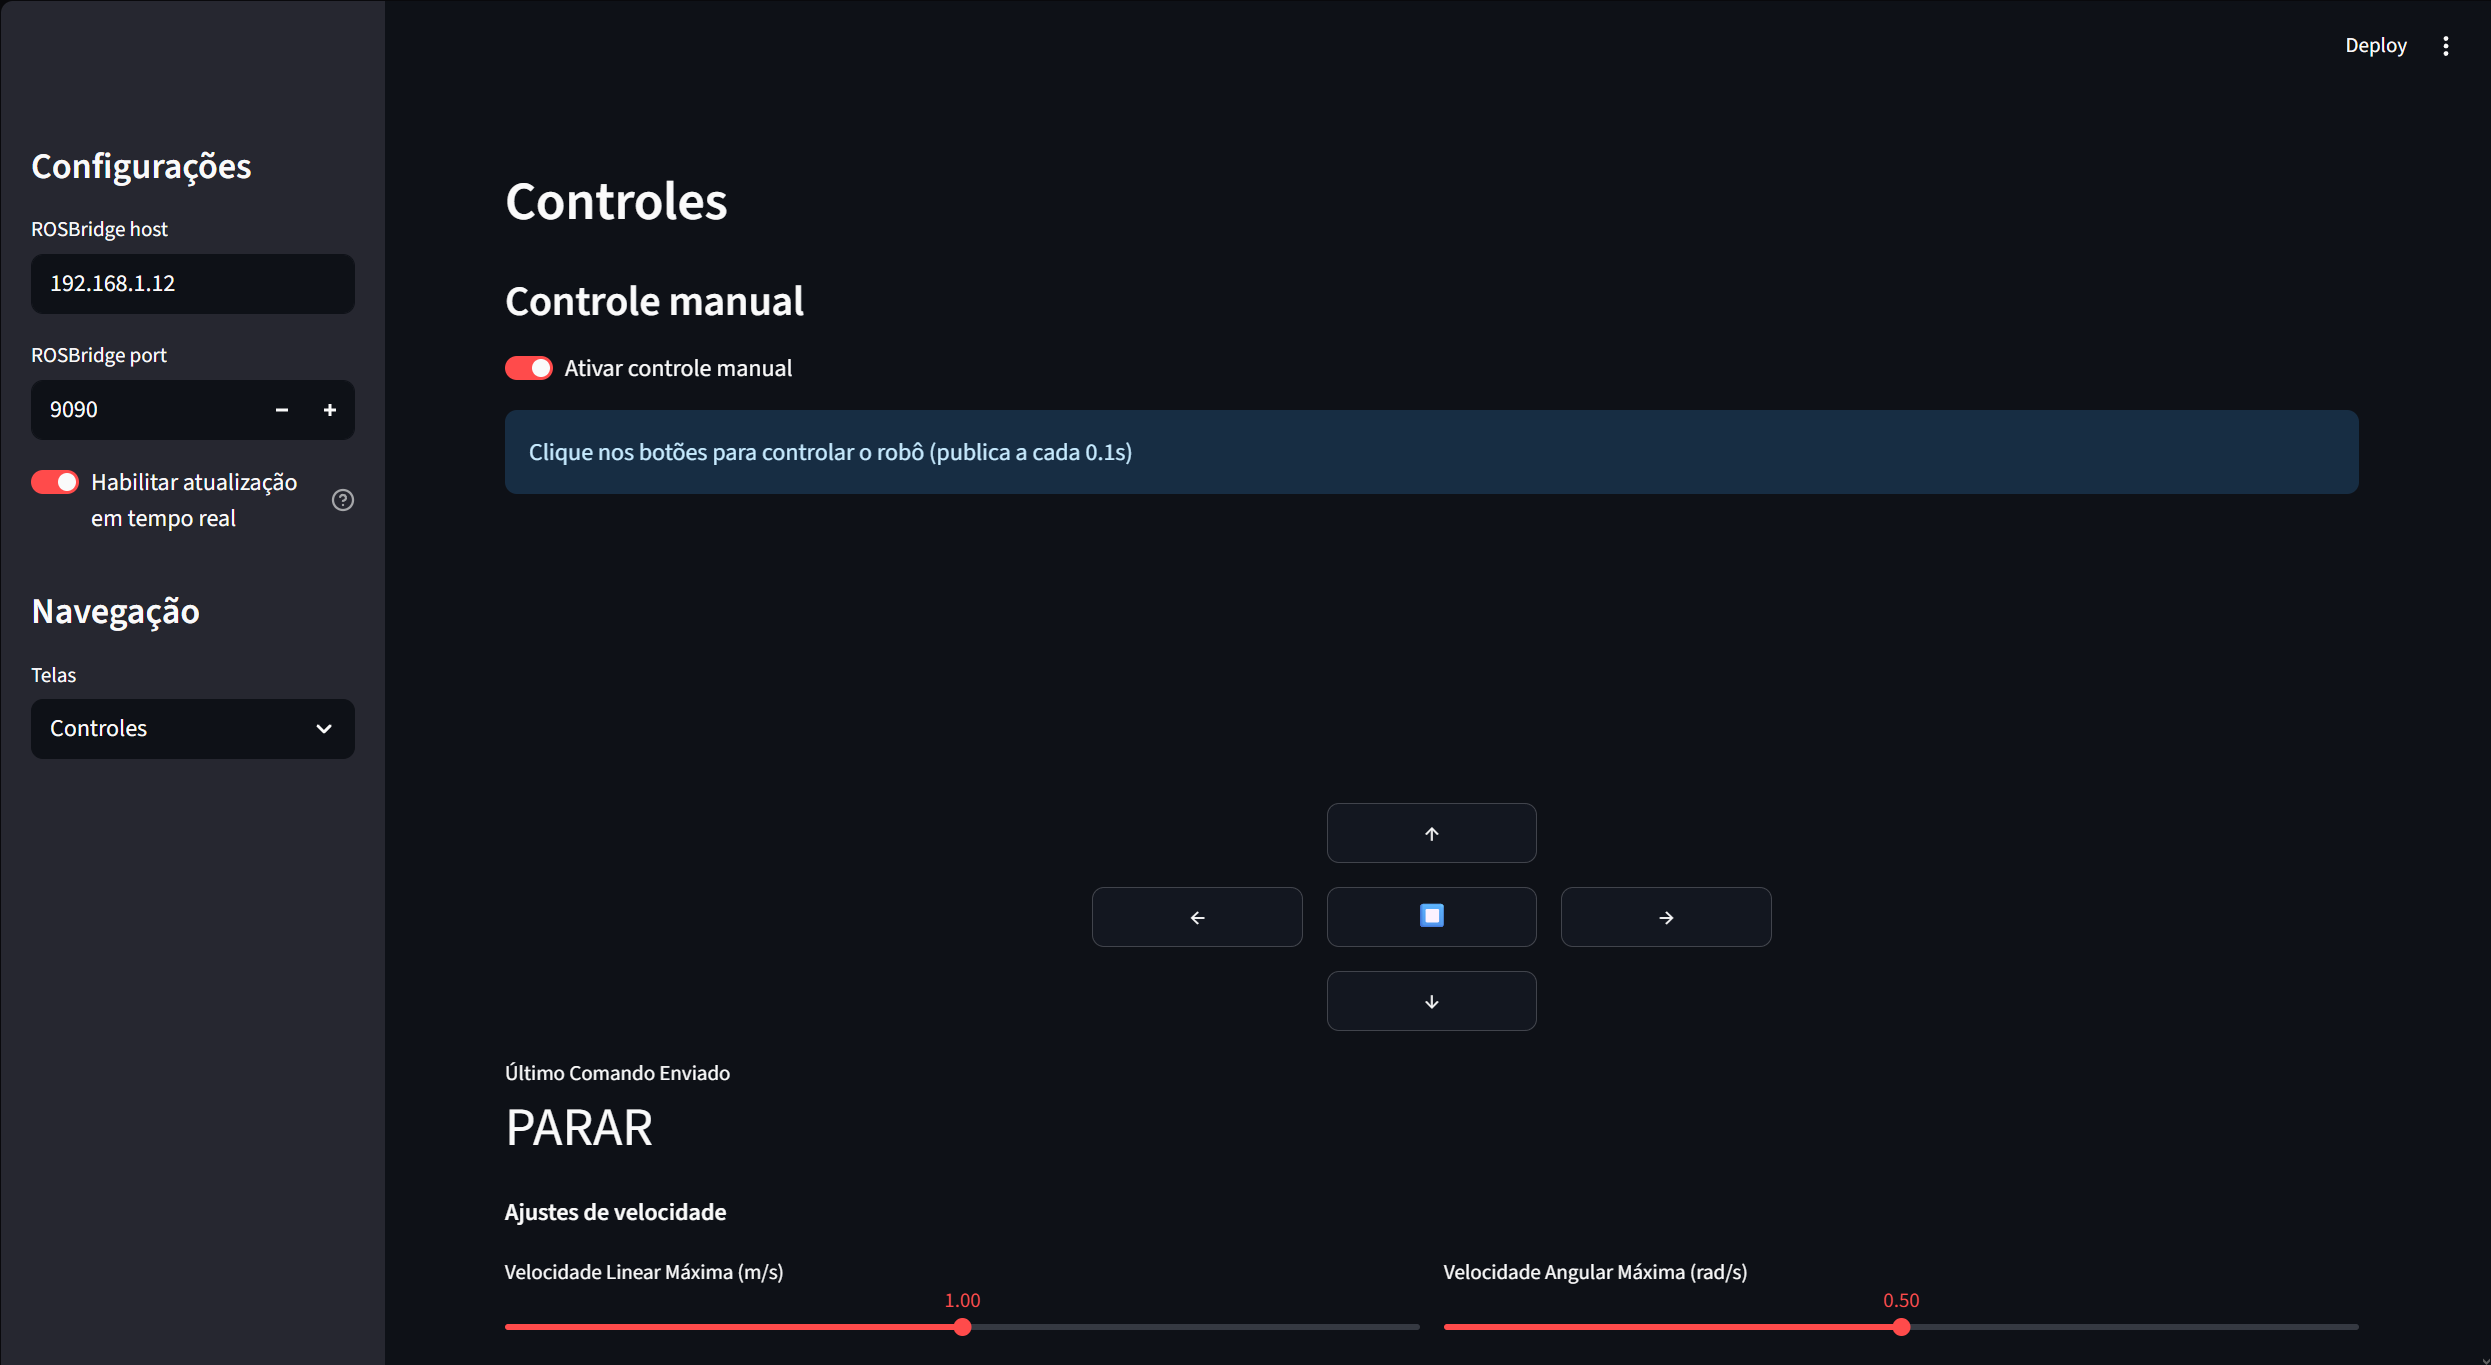
\includegraphics[width=\textwidth]{images/Controles.png}
    \vskip0.5\baselineskip
    \captionof{figure}{Módulo de controle da interface.}\label{fig:controle}
\end{center}

\begin{center}
    \includegraphics[width=\textwidth]{images/RVizControle.png}
    \vskip0.5\baselineskip
    \captionof{figure}{Envio de comandos de controle manual para o ROS.}\label{fig:rvizcontrole}
\end{center}
